\chapter{Autonomous Morphology as a Target of Learning}
\label{autonomous}

\section{Introduction}
Many morphologists in recent decades have rejected the notion of the morpheme---a concept that inextricably binds morphology to syntax and semantics---in favor of approaches that regard morphology as autonomous, i.e., as independent 
of both syntax/semantics and phonology. The principle objective of this chapter is to 
show that autonomous morphological units are legitimate learning targets for system of unsupervised morphological learning. In fact, as we will soon see, autonomous morphology is more than just legitimate; it is the only possible learning target for the unsupervised learning of morphology (ULM) as it is conventionally defined.
In the course of the discussion, we shall consider some of the more prominent theories of autonomous morphology, contrasting them with ``non-automonous'' approaches, and  noting their significance to ULM (and Multimorph in particular).


\section{The Unsupervised Learning of \textit{What}, Exactly?}
\label{sec:what-exactly}
In the ULM literature, authors often use the word \emph{morpheme(s)} 
when describing their systems' \emph{learning target(s)}, i.e., what their systems are meant to learn and 
output, as well as the features that compose their input feature vectors.
\cite{poon-et-al:2009}, for example, use two main categories 
of features, one of which they refer to as \emph{morpheme-context} features (see chapter \ref{ch:lit-review}).
\cite{goldsmith:2001, goldsmith:2006} also uses the word 
\emph{morpheme}.
The creators of Morfessor 
\citep{creutz-and-lagus:2002, 
creutz-and-lagus:2005, creutz-and-lagus:2007}
use a range of terms, including 
\emph{morpheme},
\emph{morpheme-like}, and \emph{morph}. The following quotations 
illustrate these usages (emphasis added):
\begin{exe}
\ex ``The model presented in this 
work provides a good means for the segmentation of words into 
\textbf{morphemes} \citep[][p. 6]{creutz-and-lagus:2007}. 
\ex``[W]e have demonstrated how the meaning and form of 
\textbf{morpheme-like} units can be modeled in a 
morphology induction task\dots'' \citep{creutz-and-lagus:2005}.
\ex``The lexicon contains one entry for each distinct \textbf{morph} 
(morph type) in the 
segmented corpus'' \citep[][p. 9]{creutz-and-lagus:2007}. 
\end{exe}
Creutz and Lagus seem to prefer the more general, theory-neutral term \emph{morph} 
in more formal or technical contexts. Indeed,
of the above three terms, they probably use 
\emph{morph} most frequently.

Moreover, ULM researchers virtually never specify what they mean
when they use the word \emph{morphology}, even though there
are currently at least two fundamentally different schools of thought concerning the nature of morphology. These are the 
the \emph{morpheme-based} and \emph{lexeme-based} views, to borrow the labels that \cite{aronoff:1994} has assigned 
to these categories. The lexeme-based view, which has been gaining momentum in recent decades \citep{anderson:2017},
is that there exists an \emph{autonomous} layer of morphology, a layer that mediates between (morpho-)syntax
and phonological realization, but has neither meaning nor phonologically realized form in and of itself. Proponents
of lexeme-based morphology thus do not believe in pairings of form and meaning, i.e., \emph{morphemes}, as fundamental linguistic
units \citep{anderson:2015}. We will further discuss the notion of autonomous morphology in section~\ref{sec:morpho-theories}.

One's morphological theory affects the way in which one interprets the output of a ULM  system. 
If one describes a ULM  system and its learning task in terms of 
morpheme-based morphology, one must also struggle to 
describe its output as consisting of morphemes, as do, for example, 
\cite{creutz-and-lagus:2007,creutz-and-lagus:2005}. In contrast, under a 
lexeme-based theory, one would view the output of a ULM  system as 
consisting of \emph{autonomous} morphological units, i.e., 
expressly non-morpheme units. 
Thus, one's theory of morphology makes an implicit claim about the output of 
his/her ULM  system.

The output of any machine learning system depends to 
a great extent on the nature of its input, which, in the case of the 
\emph{unsupervised} learning of morphology, 
depends to a large extent on with the meaning of ``unsupervised.'' 
All of the major ULM  
systems take as input a list of independent tokenized words 
\citep[e.g.,][]{goldsmith:2001,baroni-et-al:2002,creutz-and-lagus:2005,poon-et-al:2009}
Thus, a convention seems to have emerged whereby, in the 
case of ULM , the meaning of \emph{unsupervised} includes a
requirement that each word be free of morphosyntactic 
or semantic information. In practice,
this means being entirely free of context. I am 
not aware of a ULM system that extracts features from the raw context surrounding a given word, i.e.,
the unanalyzed words adjacent to the unanalyzed word question. It seems doubtful
that such a context could be helpful to a machine learner. 
It would probably have to be abstracted and categorized 
(i.e., annotated) in order
for it to be helpful to a system.

%Because morphemes are irreducible and arbitrary pairings of form and meaning
%but in 
Classical morphemes are (irreducible) pairings of form and meaning.
In order to learn morphemes, therefore, a system needs to learn meaning. But a ULM system does not have access to
the contexts of its input words, as its input is a list of independent word tokens, and thus it cannot learn
meaning.
% because the input to ULM systems is a list of contextless tokenized words. 
% learning meaning without contextual information. And since the input to a ULM 
% a ULM system consists of independent words without contextdoes not have access to context, it simply 
cannot learn classical morphemes. 
A ULM system might learn 
character subsequences that happen to resemble
 classical morphemes \emph{in form}, but only because morphological systems
do tend to cooperate with syntax/semantics in some way, and in some 
 cases this cooperation is more transparent and straightforward than
 in others.  However, this ULM system would nevertheless be oblivious to the actual meanings
 of these pieces of form. Meaning is an essential component of the classical morpheme, and because
 meaning depends on context, there is no way to induce classical morphemes from contextless words.
Therefore, ULM systems, particularly those which learn solely from 
from lists of raw, contextless words, simply cannot learn 
\emph{morphemes} in the strict sense of the term.

Consider, for example, Linguistica, the seminal 
ULM  system developed by \cite{goldsmith:2001, goldsmith:2006}. 
Linguistica finds morphological relationships by filling in 
data structures 
called \emph{signatures} as it iterates over datasets comprising many
thousands of contextless words. Each signature $\sigma$ 
comprises 
two sets, $S$ and $A$, a set of stems and a set of affixes, 
respectively.
A \emph{signature} is a pair of sets, namely a set of stems $S$ and 
a set of affixes $A$, such that each stem-affix combination in the cross 
product $S \times A$ is observed in the corpus. Additionally, $S$ and 
$A$ must each contain at least two members, with \textsc{null} being 
a permissible member, and each stem can belong to only one signature.  
For example, a signature could be the following: $S = \{ \text{act}, \text{back}, \text{mint} \}$ 
and $A = \{ \textsc{null}, \text{s}\}$. Every possible stem-affix combination is 
\begin{equation}
\label{eq:SxA}
S \times A = \{ \text{act}, \text{back}, \text{mint}, \text{act-s}, 
\text{back-s}, \text{mint-s}\}
\end{equation}
The fifth 
most common signature that Linguistica found among the words of 
\textit{Tom Sawyer} had as its affix set $\{\textsc{null}\textit{.ed.ing.s}\}$ \citep{goldsmith:2001}. 
The corresponding stem set had 14 members, though \citet{goldsmith:2001} 
does not identify the individual stems. 
In any case, the affix set \textsc{null}\textit{.ed.ing.s} represents 
a stem equivalence class. Its extraction would be an impressive achievement for any ULM system, and this
is but one of many such signatures that Linguistica has found. However, 
suppose we had no knowledge of English. It would then be impossible to deduce the nature 
of this equivalence class. We might
guess that it is a morphosyntactic category of \emph{some kind}, but since we would be ignorant
of the affixes' meanings/functions, this would be nothing more than a guess. 

An English speaker can probably deduce that \textsc{null}\textit{.ed.ing.s} are suffixes that attach to verbs,
but this it is the speaker's general competence in the language that informs this deduction, not anything in the 
signatures themselves.

Thus, although Linguistica does learn morphological equivalence classes, 
sets of stems that combine with the same affixes 
(and sets of affixes that combine with with the same stems) 
it does not learn to associate \textit{-s}, for example, 
with `3rd-person singular present-tense'. That is, it does not assign particular
meanings to the stems and affixes it discovers.
Nor would Linguistica know the particular meaning of any stem 
associated with a given affix set. 
Suppose that \{\textit{act}, \emph{jump}, \emph{laugh}\} 
was the stem set associated with \textsc{null}\textit{.ed.ing.s}. 
Linguistica would thus have learned that these stems are the same 
in a way. But Linguistica would not have learned what this 
equivalence should have signified, not would have learned the semantic 
distinctions between the members of the same equivalence set. 
That is, even though \textit{act}, \emph{jump}, and \emph{laugh} 
share the same affix set, they do not share the same meaning. 
Thus, we must conclude that Linguistica does not learn morphemes 
in the classical sense, i.e., with each morpheme being a
pairing of one form and one meaning.

To be sure, this is not a failing on the 
part of Linguistica, which is indeed an effective 
unsupervised learner of morphology. Given the definition 
of the classical morpheme and the limited nature of 
Linguistica's input, it is simply not possible for 
Linguistica to learn true morphemes. First, because 
Linguistica is an \emph{unsupervised} learner, it has 
no access to the information it would need to assign meaning to units of form.
Second, as we will see in section~\ref{sec:morpho-theories}, morphemes do not adequately 
account for the full range of morphological phenomena \citep{anderson:2017}. 
For these reasons, morphemes are not reasonable 
targets of unsupervised morphological learning.

\section{A Spectrum of Morphological Theories}
\label{sec:morpho-theories}
In the preceding section, we argued that Linguistica does not learn morphemes. The same can be said of Morfessor, 
the system of \cite{poon-et-al:2009}, and
every other ULM  system.
 But how can we say that these systems learn morphology, but not morphemes? As it turns out,
 the existence of morphemes is by no means a sure thing.  

\subsection{Stump's Taxonomy of Morphological Theories}
\cite{stump:2001}'s oft-cited taxonomy of morphological theories 
consists of four categories. These four arise from two independent 
binary distinctions, namely \emph{lexical} vs. \emph{inferential} on the hand, and \emph{incremental} vs. \emph{realizational} on the other.
 
\begin{exe}
\ex \textsc{First Distinction}: \textit{Lexical vs. Inferential} 
\begin{xlist}
	\ex \textbf{Lexical}: \textit{A word's meaning is the compositions of its components' lexical entries.}\\
	The meaning of \textit{issue-s}, for example, is determined by the lexical entries of its components \textit{issue} and \textit{-s}.
	\ex \textbf{Inferential}: \textit{A word's meaning is determined by the meanings of related words.}\\
	The meaning of \textit{issue-s} is determined by the meanings of related forms like \textit{dog-s} and \textit{bike-s},
with ``similarities of form [directly] reflecting similarities of content and vice versa'' \citep[][p. 2]{anderson:2015shorthist}. \label{ex:d-one-b}
	\end{xlist}
\ex \textsc{Second Distinction}: \textit{Incremental vs. Realizational} 
\begin{xlist} 
	\ex \textbf{Incremental}: Each affix has its own intrinsic meaning. 
	A form's morphosyntactic property set is thus built up incrementally as it acquires affixes.
	\label{ex:d-two-a}
	\ex \textbf{Realizational}: A word's set of morphosyntactic properties 
	licenses a particular configuration of morphological exponents 
	(i.e., usually affixes of some sort). 
	\end{xlist}
\end{exe}

By cross-combining the options of first distinction with those of the second, 
\cite{stump:2001} derives four categories of morphological theories. 
\emph{Lexical-Incremental} and \emph{Lexical-Realizational} theories 
on the one hand, and on the other, \emph{Inferential-Incremental} and 
\emph{Inferential-Realizational} theories. However, \citet{anderson:2017} 
notes that most theories fall into the \emph{Lexical-Incremental} and 
\emph{Inferential-Realizational} categories. Indeed, these are the two are 
the most extreme of the four categories in that they are entirely antithetical. 
The ongoing debate over the nature and status of morphology can largely 
be framed in terms of the opposition between these two categories. 

The distinction between \emph{Lexical-Incremental} 
and \emph{Lexical-Realizational} 
theories is essentially the same as the distinction 
that \cite{aronoff:1994} draws
between \emph{morpheme-based} and \emph{lexeme-based} 
views of morphology. Morpheme-based approaches regard 
the classical morpheme as the seat of meaning.
The concept of the morpheme and morpheme-centered morphological analysis
was developed by Bloomfield in the 1920s and 1930s by
\citet{bloomfield:1926, bloomfield:1933} and honed by his 
successors in the descriptivist program, e.g., 
\cite{hockett:1947} and \cite{harris:1955}.
It was \citet[][p. 161]{bloomfield:1933} who famously wrote, ``A linguistic form 
which bears no partial phonetic-semantic resemblance to any other form is a \emph{simple} form or \emph{morpheme}'' (emphasis in the original). 
That is, a morpheme, as a pairing of a form and a meaning, is a fundamental unit; it cannot be analyzed into smaller units
of form and meaning.
Moreover, Bloomfield and the descriptivists maintained that
each \emph{complex form}, i.e., each word comprising 
two or more morphemes, was \emph{exhaustively decomposable} 
into morphemes. That is, every phonological segment
in a given word had to be either a morpheme or part of a morpheme. 

The influence of Bloomfield and the descriptivists
cannot be easily underestimated. Bloomfieldian concepts and methods 
pervade introductory linguistics courses and textbooks, both at
the undergraduate and graduate level. Any introductory text containing 
a unit on morphological analysis is going to present a methodology that 
is essentially Bloomfieldian \citep{anderson:2017}.
It is therefore perhaps no surprise that
computational linguists, including researchers in the field of ULM, 
tend to presume
the reality of Bloomfieldian morphemes and the soundness of a 
Bloomfieldian view of morphology. The Bloomfieldian approach is essentially
the lexical-incremental approach.

By contrast, lexeme-based approaches (also called \emph{word-based} 
approaches) consider the seat of meaning to be the whole word rather than its components. According to this view, the component 
parts of a complex word do not have their own predetermined meanings. 
Rather, 
there is a buffer layer between the level of phonological form and the level of
syntax/semantics. This
buffer consists of morphological rules that map from raw phonological 
strings to meanings.
Paridigm Function Morphology, a lexeme-based theory developed by \citet{stump:2001}, 
posits a morphological architecture consisting of two kinds of paradigms: a \emph{content} paradigm and a \emph{form} paradigm.
The cells of the content paradigm are related to those of the form paradigm via
\emph{paradigm functions}.
A paradigm function follows the template
%\eqref{eq:PF}, 
\begin{equation}
\label{eq:PF}
	\text{PF}\langle \text{L},\sigma \rangle = \langle \text{X}, \sigma^\prime \rangle
\end{equation}
where the lefthand side represents a particular cell in the 
content paradigm, and the righthand side a particular form-paradigm cell.
In particular, $\text{L}$ is a lexeme, and $\text{X}$ is a stem, that is, the form correspondent of $\text{L}$. 
The morphosyntactic property set associated with content cell and form cell are $\sigma$ and 
$\sigma\prime$, respectively. In the canonical case, there is a one-to-one
correspondence between content cells and paradigm cells, and 
$\sigma = \sigma^\prime$.
Often, however, the mapping between content and form cells is 
not one-to-one, $\sigma \ne \sigma^\prime$, such as in cases of
\emph{syncretism}, wherein the mapping from content to form cells is many to one. 
Consider, for example, table 
\ref{tab:engverbpres}, which shows both the content and form paradigms 
for the English lexeme \emph{kick} in the simple present tense.
The content paradigm has six cells, one for each combination of \textsc{person} 
and \textsc{number}, while the form paradigm has only two, one for the 
form that has no suffix (\textit{kick}) and the other for the form 
that ends in \textit{-s}, namely \textit{kicks}. 
 
\begin{table}[t]
\setlength{\extrarowheight}{6pt}
\centering
\begin{tabular}{ccc}
\toprule
Content Paradigm & Form Paradigm & Realization \\% inserts table
\midrule %heading
$\langle \textsc{kick}, \{ \textsc{p:1}, \textsc{n:}\text{sg} \}\rangle $ & \multirow{5}{*}{\raisebox{-32pt}{$\Bigg\langle \textsc{kick}, 
\Big\{ \big((\textsc{p:}\text{1}\vee\text{2}) \land (\textsc{n:}\text{sg} \vee \text{pl})\big) 
\vee (\textsc{p:}\text{3}\land \textsc{n:}\text{pl}) \Big\} \Bigg\rangle$}} 
& \multirow{5}{*}{\raisebox{-20pt}{kick}} \\ \cmidrule{1-1}
$\langle \textsc{kick},\{\textsc{p:2}, \textsc{n:}\text{sg}\}\rangle$  &\\ \cmidrule{1-1}
$\langle \textsc{kick}, \{\textsc{p:1}, \textsc{n:}\text{pl}\}\rangle$  & \\ \cmidrule{1-1}
$\langle \textsc{kick}, \{\textsc{p:2}, \textsc{n:}\text{pl}\}\rangle$ &  \\ \cmidrule{1-1}
$\langle \textsc{kick}, \{\textsc{p:3}, \textsc{n:}\text{pl}\}\rangle$ & \\ \midrule
$\langle \textsc{kick}, \{\textsc{p:3}, \textsc{n:}\text{sg}\} \rangle$ & $\langle\textsc{kick}, \{\textsc{p:3}, \textsc{n:}\text{sg}\}\rangle$  & kicks \\
\bottomrule
\end{tabular}
\caption{Dual-paradigm analysis of the English present tense}
\label{tab:engverbpres}
\end{table}

Notice the unnaturalness of the two morphosyntactic classes in
the form-paradigm column in table \ref{tab:engverbpres}.
Classes like these abound in morphology.  
They are unnatural in that they are not motivated by morphosyntactic properties. Thus, from a morphosyntactic
perspective, they are quite arbitrary.
There is no reason to put the third-person singular alone in one class and all of the other combinations, 
including the other singular categories as well as third-person plural, together in the other class. Such classes help motivate 
a theory of an \emph{autonomous} layer of morphology, that is, a layer responsible 
for mapping from the content level to the phonological, but does so according 
to its own terms.

Surface forms are realized phonologically by \emph{realizational rules}, which 
are functions that map from form cells (for example, those in the second column in table~\ref{tab:engverbpres})
to fully realized phonological forms (the third column in table~\ref{tab:engverbpres}). 
In fact, each realizational rule is a bijection: Every 
distinct phonological form implies the existence of a unique corresponding cell in 
the form paradigm, and conversely, each distinct form cell implies the existence of 
a distinct corresponding phonological form. The
content-paradigm cells are not directly connected to the realizational rules of 
the phonological level because the form paradigm acts as an 
intervening layer---a layer of autonomous morphology---between the 
content paradigm and the level of phonological realization. 
Thus, according to Paradigm Function Morphology, the content paradigm cannot directly influence phonological form. 

Realizational rules come in two varieties:
\emph{rules of exponence} and \emph{rules of referral}. Rules of exponence, as exemplified in \eqref{eq:roexp}, describe the 
realization of surface forms from morphological \emph{exponents}. They take the form 
$\text{X},\text{C},\sigma \to f(\text{X})$, where X is the stem, C is the lexical category of X, 
$\sigma$ is a morphosyntactic property set,  and $f(\text{X})$ is the morphological operation to be performed 
on X, as in ``Xs'' (addition of an \emph{-s} suffix). The two rules of exponence in \eqref{eq:roexp}  
correspond to the two forms 
of English present-tense verbs (see table~\ref{tab:engverbpres}). 
\begin{align}
\label{eq:roexp}
	\text{X},\text{V},\sigma\text{:} \quad
	\{ \textsc{pers:3}\text{,} \land \textsc{num:}\text{sg,} \land \textsc{tns:}\text{pres} \} &= \text{X}s \\ 
	%\label{eq:roexp1}
	\text{X},\text{V},\tau\text{:} \quad
	%\{((\textsc{pers:}\text{1}\vee\text{2}) \land (\textsc{num:}\text{sg}\vee\text{pl})) \vee (\textsc{pers:}3 \vee \text{sg})\} 
	%\Bigg\langle \textsc{kick}, 
\Big\{ \big((\textsc{pers:}\text{1}\vee\text{2}) \land (\textsc{num:}\text{sg} \vee \text{pl})\big) 
\vee (\textsc{pers:}\text{3}\land \textsc{num:}\text{pl}) \Big\} %\Bigg\rangle 
&= \text{X} 
\end{align}
where $\text{V}$ (\textit{verb}) is the lexical category of \textit{X},
%, which is  in this case is \textsc{verb}, 
and $\sigma$ and $\tau$ are distinct morphosyntactic property sets. 

By contrast, a rule of referral redirects the word formation process to a different ``rule block,'' i.e.,
a different morphosyntactic property set. Such a rule takes the form 
\begin{equation}
\label{eq:ror}
\text{X}, \text{C}, \sigma \to \, \tau \, \text{in Block \textit{A}}
\end{equation}
Here, X again is a stem, 
C its lexical category, and $\sigma$ its morphosyntactic property set. However, instead of the usual $f(\text{X})$ 
to the right of the arrow, we have in this case a redirection to a 
different morphosyntactic property set in a different rule block. (The \textit{A} in ``Block A'' 
is a purely arbitrary label in this case.) Stump cites the English perfect participle 
to exemplify rules of referral. That is, for many lexemes, the form of the 
past participle is identical to the simple-past form, e.g., \textit{raked}. 
These participles would be formed through a rule of referral, i.e., one that 
says, in effect, ``To get your perfect participle form, imagine that you 
were a past-tense form, and proceed accordingly.''  We will revisit the English 
perfect participle when we discuss morphomes 
in section~\ref{sec:the-morphome}.

Paradigm Function Morphology is an example of a morphological theory that involves an intermediate layer between
meaning (i.e., content) and phonological form---and thus an indirect relationship between
meaning and form. In the case of Paradigm Function Morphology, this intermediate
level is of the form paradigm. It interacts with the semantics and phonology 
via paradigm functions and rules of exponence, respectively,
but it is nonetheless independent of both the semantics and the phonology and thus a layer of \emph{automonous} morphology.  

In his influential book \textit{Morphology By Itself} (1994), Aronoff 
introduces the concept of the \emph{morphome}, which he
defines as a function ``that is neither 
syntactic nor phonological'' \cite[][p. 25]{aronoff:1994},
as well as a
``mapping from morphosyntax to phonological realization'' \citep[][p. 25]{aronoff:1994}. 
It is related
to the cells in Stump's form paradigm (see table~\ref{tab:engverbpres}), 
but it is also more complex. It is to the morphome that we turn next.

\subsection{The Morphome}
\label{sec:the-morphome}
The morphome has sparked a 
great deal of research since Aronoff introduced it in 1994. Researchers
such as \cite{maiden:2005, maiden:md:2016}, \cite{round:2009, round:2011, 
round:2012, round:2015, round:md:2016}, \cite{oneill:2014b,oneill:2018}, and \cite{bonami:2008, bonami:2010}, to name 
a few---have found examples of morphomicity in a wide variety of 
languages and have thereby helped to flesh out the notion of the morphome.
Round, for instance, in \cite{round:2009} and subsequent works, 
presents a complete morphome-based analysis of the morphology of 
Kayardild, a nearly extinct language of northern Australia. 

\subsubsection{Morphormic Representations}
Round expresses a word's \emph{morphomic representation} as a pair 
consisting of a particular lexical item and a particular set of properties.
\cite{round:2011} argues that such pairs can be either inflectional 
 or derivational in nature, and moreover, that the same morphome can fill 
 both inflectional and derivational roles. In English, for example, \emph{-s} 
functions as the \textsc{3.sg} present-tenxe suffix for verbs and as the \textsc{pl} 
 suffix for nouns, both of which are inflectional, but it can also serve a derivational 
 role as the possessive clitic, e.g.,
 {\emph{The girl\textbf{'s} new bicycle}, as well as a
 cliticization of the copula, e.g., \emph{The girl's bicycle\textbf{'s} new} (`The girl's bicycle \emph{is} new').

%  \begin{exe} 
% \emph{This is the \textbf{girl's} new bicyicle}
%  \ex This is the \textbf{girl's} new bicyicle.
%  \end{exe} 
%  and the \textsc{3.sg.pres} clitic, as in
%  \begin{exe} 
% % \ex \emph{The girl's\textbf{bicycle's} new.} 
%  \ex The girl's\textbf{bicycle's} new.
%  \end{exe} 
 Hebrew also has morphomes that ``cross the inflectional--derivational divide,'' 
 as Round puts it \citep[][p.14]{round:2015}. This inflectional--derivational 
 duality will prove useful to us in section \ref{sec:heb-example}, where we will 
 examine a case of syncretism among certain inflectional and derivational suffixes in Modern Hebrew.
  
  But first we must establish some notation. 
  One of Round's contributions is his rigorously formalized descriptions of 
  morphomic phenomena. In \citet{round:2011}, for instance, 
  he expresses the \emph{morphomic representation} of a word 
  \textit{w} as a function $\mu{\textsc{word}}$ that 
  takes as input a pair of items, the precise nature
  of which depends on whether one is dealing with inflectional or 
  derivational morphology. In the former case, the input pair comprises 
  a lexeme $\lambda$ and a morphosyntactic property set ($\sigma$); in the latter, 
  it consists of a root $\rho$ and a derivational property set $\delta$. 
  Both cases are presented in table~\ref{tab:morphreps}. If the word \textit{w} 
 is complex, its morphomic representation $\mu{\textsc{word}}$ 
  can be decomposed (or factorized) into constituents as  
  $\langle  \mu_{I} \dots \mu_{2}, \mu_{1}, x \rangle$, where $x$ 
  is some kind of initial form, such as a root or a stem. The elements in the sequence 
  $ \mu_{I} \dots \mu_{2}, \mu_{1}$ are each morphomes, 
  which, according to \citet{round:2015}, can be viewed as operations, 
  such that each applies rightward, starting with the lowest index, and progressing upward
  to index $I$.
  
  Whereas the $\mu$'s in table~\ref{tab:morphreps} represent 
  morphomes and morphomic representations, the $\Phi$'s represent 
  phonological units, i.e., phonological operators. Phonological operators are functions that realize morphomes as phonological entities. 
  Like the $\mu$'s, 
  the $\Phi$'s are indexed. But notice that the  indices on the $\Phi$'s $(1,2,\dots,J)$ 
  do not necessarily match those on the $\mu$'s $(1,2,\dots,I)$. This is to say that
the correspondence between 
  morphomes and phonological units is not always one-to-one, a point that Round is careful to make in 
  in \cite{round:2015}. This point
  will also prove to be important for our analysis of certain Hebrew 
  suffixes in section~\ref{sec:heb-example}. Because, according to Round, there does not need to be a one-to-one correspondence between morphomes and phonological operators, it is possible that two morphomes, for instance, should map to a single phonological operator. 

\begin{table}[t]
 \setlength{\extrarowheight}{6pt}
\centering
\begin{tabular}{l c c c}
\toprule
    & \makecell{Lexical\\(Output)} & \makecell{Morphomic}  & \makecell{Phonological\\(Input)}  \\
   % & (Input)	 &        	&  (Output) \\
\midrule
\multirow{2}{*}{Inflection} & \multirow{2}{*}{$\langle \lambda,\sigma \rangle$} & $\mu{\textsc{word}}(\lambda,\sigma)$ & $\Phi{\textsc{word}}(\lambda,\sigma)$\\     
    				&  &  $\langle  \mu_{I} \dots \mu_{2}, \mu_{1}, x \rangle$ & 
				$\langle  \Phi_{J} \dots \Phi_{2}, \Phi_{1}, x \rangle$ \\ \midrule
\multirow{2}{*}{Derivation} & \multirow{2}{*}{$\langle \rho,\delta \rangle$} & 
$\mu{\textsc{word}}(\rho,\delta)$ & 
$\Phi{\textsc{word}}(\rho,\delta)$ \\
    				& & $\langle \mu_{I} \dots \mu_{2}, \mu_{1}, x \rangle$ & $\langle \Phi_{J} \dots \Phi_{2}, \Phi_{1}, x \rangle$ \\[0.5ex]
\bottomrule
\end{tabular}
\label{tab:morphreps}
\caption{Three levels of representation}
\end{table}

Consider the morphomic representation $\mu{\textsc{word}}(\lambda,\sigma)$.
Suppose the morphosyntactic property set $\sigma$ were replaced with a different such set, namely $\tau$. 
Such a swap could result in a different phonological realization, but not necessarily. 
That is, $\Phi{\textsc{word}}(\lambda,\tau)$ could very well be identical to 
 $\Phi{\textsc{word}}(\lambda,\sigma)$. One sees this kind of identity in English
 present-tense verbs, as exemplified in table~\ref{tab:engverbpres}. Every form is identical except the third-person singular, which takes the \textit{-s} suffix.

\subsubsection{A central morphomic maxim} A central maxim 
of morphomic theory is that
\emph{identity at the phonological 
level entails identity at the morphomic level} \citep{round:2011}. 
That is, if two 
or more words share a particular subsequence of phonemes 
(or symbols, etc.), then their respective morphomic representations 
must all share a particular morphome, since it is the shared 
morphome that gives rise to the shared subsequence at the 
phonological level. This maxim is crucial for the purposes 
of ULM because it licenses an algorithm to identify 
morphological units solely on the basis of similarities in 
form, irrespective of meaning.

Suppose, for example, that 
\begin{align*}
%$\lambda &= \textsc{kick}$\\
%$\sigma &=$ $\{\text{\textsc{pers}:1, \textsc{num}:pl, \textsc{tns}:pres} \}$\\
%$\tau &=$ $\{\text{\textsc{pers}:2, \textsc{num}:sg, \textsc{tns}:pres}\}$\\
\lambda &= \textsc{kick} \\%\text{, and}\\
\sigma &= \{\text{\textsc{pers}:1, \textsc{num}:pl, \textsc{tns}:pres} \} \\%\} \text{, and}\\
\tau &=\{\text{\textsc{pers}:2, \textsc{num}:sg, \textsc{tns}:pres}\}
\end{align*}
Even though the morphosyntactic property sets $\sigma$ and $\tau$ are very much different,
the phonological representations of $\langle \textsc{kick}, (\lambda,\sigma) \rangle$
and $\langle \textsc{kick}, (\lambda,\tau) \rangle$ are identical. 
That is,
\begin{align*}
\Phi\textsc{kick}(\lambda,\sigma) \quad &= \quad \text{\textipa{/kIk/}} \\%\text{, and} \\
\Phi{\textsc{kick}}(\lambda,\tau) \quad &= \quad \text{\textipa{/kIk/}} %\text{.}
\end{align*} 
%Thu because 
%\begin{equation*}
By the above maxim, because
$\Phi{\textsc{kick}}(\lambda,\sigma) =  \Phi{\textsc{kick}}(\lambda,\tau)$, we can say that  %\\ \text{, and} \\
%\end{equation*}
%we have that 
\begin{equation*}
\mu{\textsc{kick}}(\lambda,\sigma) = \mu{\textsc{kick}}(\lambda,\tau) %\text{.}
\end{equation*}
That is, because these two instances of \textsc{kick} are identical in 
phonological form, their morphomic representations must also be identical. 
%In other words, they must have the \emph{same} morphomic represention. 
If the 
phonological forms were only partially identical, their morphomic 
representations would also be partially identical. For example, if they 
shared a suffix, then the identity at the mormophic level would 
be the morphome corresponding to this suffix.

\subsubsection{A Taxonomy of Morphomes}
Another contribution of Round is his taxonomy of morphomes, which 
classifies morphomes according to the types of groups they engender. 
That is, if we think of morphomes as relations, we can think of them as 
sets whose members all are alike in a particular way. \cite{round:2015, round:md:2016} 
classifies morphomes according to the nature of this similarity. That is, 
according to Round, there are different types of form-based similarity; i.e., different ``aspects of form'' that are 
shareable \citep[][p.230]{round:md:2016} and these different shareable aspects of form correspond to different types of morphomes. 
This sort of taxonomy will prove useful when we discuss the 
limitations on unsupervised morphological learning, i.e., what a ULM 
system can and cannot learn given the limited nature of its input.

Round's taxonomy comprises three categories, namely 
\textit{\textbf{rhizo}morphomes}, \textit{\textbf{meta}morphomes}, 
and \textit{\textbf{mero}morphomes}. 
Rhizomorphomes and metamorphomes both transcend the confines of 
particular lexemes and are thus both
rather abstract. Meromorphomes, in contrast, correspond to``concrete'' 
pieces of form. They are the raw material from which paradigms are constructed. 
Of these three, metamorphomes and meromorphomes will be most 
relevant to the present discussion, but we shall touch on rhizomorphomes briefly 
before proceeding to metamorphomes and meromorphomes.

\paragraph{Rhizomorphomes.} A rhizomorphome is a set of stems or roots
 whose members all take the same set of inflectional exponents. They include, for example,
 noun declensions, such as Latin's third declension.

\paragraph{Metamorphomes.} A metamorphome is a pattern of stem 
equivalence that spans multiple paradigms 
(and thus multiple lexemes). See, for example, tables~\ref{subtab:digo}
and \ref{subtab:crezco}, which demonstrate the L-morphome, a prominent 
metamorphome in Romance languages \citep{maiden:2005}. Although the 
lexemes defer in these tables, the morphome is the same. This is because 
the morphome is not the particular stem in either table, but rather the 
\emph{pattern} of stem equivalence. In this case, the equivalence class 
forms  an ``L''-shape when the paradigm cells are arranged as in tables~\ref{subtab:digo} 
and \ref{subtab:crezco}.
\begin{table}[t]\label{tab:l-morphome}
 \setlength{\extrarowheight}{6pt}
\centering % used for centering table
\subtable[\textit{decir} `to say' \label{subtab:digo}]{
\begin{tabular}{l c c c c c c} % centered columns (4 columns)
\toprule
	& \textsc{1.sg} & \textsc{2.sg} & \textsc{3.sg} & \textsc{1.pl} & \textsc{2.pl} & \textsc{3.pl} \\
\cmidrule{2-7}
\textsc{pres ind} & \textbf{dig}o & dices & dice & dec\'imos & dec\'is & dicen  \\ 
\textsc{pres subj}& \textbf{dig}a & \textbf{dig}as & \textbf{dig}a & \textbf{dig}amos & \textbf{dig}a\'is & \textbf{dig}an \\
\bottomrule
\end{tabular}
}
\vspace{7pt}
\subtable[\textit{crecir} `to grow' \label{subtab:crezco}]{
\begin{tabular}{l c c c c c c} 
\toprule
	& \textsc{1.sg} & \textsc{2.sg} & \textsc{3.sg} & \textsc{1.pl} & \textsc{2.pl} & \textsc{3.pl} \\ % inserts table
\cmidrule{2-7}
\textsc{pres ind} & \textbf{crezc}o & creces & crece & crecemos & crece\'is  & crecen   \\
\textsc{pres subj} & \textbf{crezc}a & \textbf{crezc}as & \textbf{crezc}a & \textbf{crezc}amos & 
\textbf{crezc}a\'is & \textbf{crezc}an   \\
\bottomrule
\end{tabular}
}
\caption{The stem \textit{crezc-} `say' is an L-morphome in Spanish.}
\end{table}

One of the hallmarks of morphomes in general is that they tend to
correspond to unnatural combinations of morphosyntactic 
properties \citep{aronoff:md:2016}, and the L-morphome is no exception. 
The L-morphome can be defined as the \emph{set} of verb 
stems that coincide with the following highly unnatural morphosyntactic property set:
\begin{equation}
\{ \text{\textsc{tns}:pres, \textsc{mood}:subj}\} \vee \{\text{\textsc{tns}:pres},\text{\textsc{mood}:ind},\text{\textsc{pers}:1},\text{\textsc{num}:sg}\}
\end{equation}

Another example of a metamorphome is the English perfect participle, which was first 
identified as a unified, albeit complex, morphome by \cite{aronoff:1994}. The term \emph{perfect participle} 
itself refers not to a particular syntactic category, but 
to a class of 
forms whose members 
can serve a variety of  syntactic purposes. For instance, a perfect participle can be combined
with inflections of \emph{have} to form the perfect tenses, but also with 
\emph{was} to express the passive voice. 

In each of the examples~(\ref{ex:pastpart:kick}), (\ref{ex:pastpart:write}), and (\ref{ex:pastpart:sing}), a present-perfect verb is identical to 
a passive verb.

\begin{exe}
\label{ex:pastpart}
	\ex Root ($\rho$): $\surd$\textsc{kick}
		\begin{xlist} \label{ex:pastpart:kick}
		\ex \textsc{Perfect:} Susan has kicked the ball. \label{ex:pastpart:kick:perf}
		\ex \textsc{Passive:} The ball was kicked by Susan.\label{ex:pastpart:kick:pass}
		\end{xlist}
	\ex Root ($\rho$): $\surd$\textsc{write}
		\begin{xlist} \label{ex:pastpart:write}
		\ex \textsc{Perfect:} Susan has written the report. \label{ex:pastpart:write:perf}
		\ex \textsc{Passive:} The report was written by Susan. \label{ex:pastpart:write:pass}
		\end{xlist}
	\ex Root ($\rho$): $\surd$\textsc{sing}
		\begin{xlist} \label{ex:pastpart:sing}
		\ex \textsc{Perfect:} Susan has sung the hymn. \label{ex:pastpart:sing:perf}
		\ex \textsc{Passive:} The hymn was sung by Susan. \label{ex:pastpart:sing:pass}
		\end{xlist}
\end{exe}
However,
from a hyper-root perspective, so to speak, we see that the precise \emph{instantiation} of the sameness varies from root to root.  
Table~\ref{tab:engpastpart} summarizes five varieties of the metamorphome $\mu{\textsc{perf}}$.\footnote{Note that this table
does not express the full variety of $\mu{\textsc{perf}}$'s realizations, as ablaut can take a number of different shapes.}
\begin{table}[!t]
\centering
\setlength{\extrarowheight}{8pt}
\begin{tabular}{c c c c c}
\toprule
& & & \multicolumn{2}{c}{Syntactic Function} \\[-1ex] 
Root & Type & Form & Perfect & Passive  \\ [0.5ex]
\midrule
\textsc{dance} & -(e)d & danced & (has/had) danced & (was) danced \\
\textsc{leave} & -t & left & (has/had) left & (was) left \\ 
\textsc{write} & -en & written & (has/had) written & (was) written \\
\textsc{sing} & ablaut & sung & (has/had) sung & (was) sung \\
\textsc{break} & abluat, -en & broken & (has/had) broken & (was) broken \\
\bottomrule
\end{tabular}
\label{tab:engpastpart}
\caption{The English past-participle is a metamorphome; that is, it is a single abstract morphome instantiated across many different lexemes. Different lexemes may correspond to different stem types, which in turn take their own distinct affixes.}
\end{table}

%\begin{table}[ht]
%\centering
%  \subtable[broken\label{subtab:eng-break}]{
%    \centering
%    \setlength{\extrarowheight}{8pt}
%        \begin{tabular}{l c c }
%        \toprule
%        \multirow{2}{*}{Phonological} & \textipa{broUk} & en \\
%         & $\Phi${\textsc{stem}} & $\Phi${\textsc{en}} \\
%         
%         \multirow{2}{*}{Morphomic} & $\mu$\textsc{ablaut:o}, $\surd$\textsc{br-k} & $\mu$\textsc{en} \\
%           					& \multicolumn{2}{c}{$\mu$\textsc{perf}, $\surd$\textsc{br-k}} \\ 
%         Lexical & \multicolumn{2}{c}{$\surd$\textsc{br-k}, \{{past-perfect}$\vee${passive}\}} \\
%         \bottomrule
%                 \vspace{1pt}
%    \end{tabular}
%    }
%    \subtable[sung\label{subtab:eng-sing}]{
%    \setlength{\extrarowheight}{8pt}
%    \centering
%        \begin{tabular}{l c   }
%        \toprule
%        \multirow{2}{*}{Phonological} & \textipa{s2N} \\
%         				& $\Phi\textsc{stem}$  \\  
%        \multirow{2}{*}{Morphomic} & $\mu$\textsc{ablaut:u}, $\surd$\textsc{\textipa{s-N}}\\
%           	 & \multicolumn{1}{c}{$\mu$\textsc{perf}, $\surd$\textsc{sing}} \\ 
%	 Lexical & \multicolumn{1}{c}{$\surd \textsc{sing}$, \{{past-perfect}$\vee${passive}\}}\\
%        \bottomrule
%        \vspace{1pt}
%    \end{tabular}
%  }
%      \subtable[kicked\label{subtab:eng-kick}]{
%    \centering
%    \setlength{\extrarowheight}{8pt}
%        \begin{tabular}{l c c }
%        \toprule
%        \multirow{2}{*}{Phonological} & \textipa{kIk} & -d \\
%         & $\Phi$\textsc{stem} & $\Phi$\textsc{d} \\
%        $\mu$\textsc{perf}: &  $\surd$\textsc{kick} &  $\mu$\textsc{d}   \\
%        Lexical & \multicolumn{2}{c}{$\surd \textsc{kick}$, \{{past-perfect}$\vee${passive}\}}\\ 
%         \bottomrule
%    \end{tabular}
%  }
%  \label{tab:eng-perf}
%\caption{Morphomic analyses for some English past-participle forms}
%\end{table}

\begin{figure}[!b]
\begin{mdframed}
\centering
     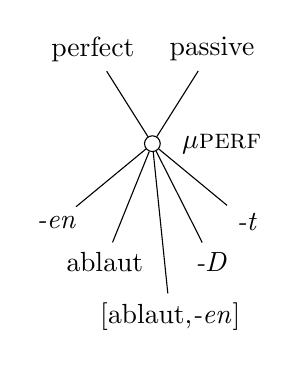
\begin{tikzpicture}[draw=black!100]
	\def \rowatticone{4.0cm}
 	\def \rowtwoht{3.5cm}
	\def \rowtwohta{3.2cm}
 	\def \rowoneht{2cm}
	\def \rowzerohta{0.8cm}
	\def \rowzeroht{0.5cm}
	\def \basementone{0.0cm}
 	\tikzstyle{ms-node}=[text centered]
 	\tikzstyle{m-node}=[circle,draw=black!100,thin,inner sep=0pt,minimum size=2mm]
	\tikzstyle{pf-node}=[text centered]
 	\tikzstyle{m-lbl}=[text width=5ex]
	\node[m-lbl] (label0) at (13ex,\rowoneht) {$\mu{\textit{\textsc{perf}}}$};
	
 	% morphosyntax
 	\node[ms-node] 	(ms0)	at (3ex,\rowtwohta)		{perfect};
 	\node[ms-node] 	(ms1)	at (13ex,\rowtwohta)	{passive};
	
 	% morphome
 	\node[m-node] 	(m0)	at (8ex,\rowoneht)		{};
	
	%phonological form
	 \node[pf-node] 	(pf0)	at (0ex,1cm)		{\textit{-en}};
 	\node[pf-node]  	(pf1)	at (4ex,\rowzeroht)		{ablaut};
 	\node[pf-node]  	(pf2)	at (9.5ex,-0.2cm)	 	{[ablaut,\textit{-en}]};
 	\node[pf-node]  	(pf3)	at (13ex,\rowzeroht) 		{\textit{-D}};
 	\node[pf-node] 	(pf4)	at (16ex,1cm) 		{\textit{-t}};	
	
 	\path (pf0)	edge	node	{}	(m0)
 		(pf1)	edge	node	{}	(m0)
 		(pf2)	edge	node	{}	(m0)
 		(pf3)	edge	node	{}	(m0)
		(pf4)	edge	node	{}	(m0)
		(m0) edge node 	{}	(ms0)
		(m0) edge node 	{}	(ms1);
		%(label0) edge node {}      (m0);	
 \end{tikzpicture}
\label{fig:ppgraph}
\caption{In the terminology of \citet{aronoff:1994}, the English perfect participle  is a \emph{polyvalent polymorphous} morphome; i.e., it has multiple functions (polyvalent) as well as multiple forms (polymorphous). The downward arcs represent form types, each of which is a \emph{meromorphomes.}}
\end{mdframed}
\end{figure}

\paragraph{Meromorphomes.} Whereas rhizomorphomes and metamorphomes 
transcend the realms of individual lexemes and paradigms and thus highly 
abstract, meromorphomes are comparatively concrete, as they 
correspond to particular parts of word forms. Meromorphomes, it must be said, 
are technically not the word parts themselves, since all morphomes reside at the 
morphomic level rather than the phonological, or surface, level \citep{round:2011}. 
Even so, meromorphomes map directly onto phonological forms, and 
are thus more closely associated with phonological forms than rhizomorphomes 
or metamorphomes. Indeed, both rhizomorphomes and metamorphomes are 
composed of meromorphomes, since, at some point, the abstract, trans-lexemic 
types of morphomes must interact with specific phonological forms. 

For instance, in English perfect participles, each individual root, e.g., \textit{s-\textipa{2N}}, 
\textit{br-k}, \textit{\textipa{kIk}}, etc., is a meromorphome, as is each suffix (e.g., \textit{-ed}, \textit{-en}, etc.}
and each distinct variety of ablaut (e.g., \textit{br\textbf{ea}k/br\textbf{o}ken}, \textit{s\textbf{i}ng/s\textbf{u}ng}, etc.) is also a meromorphome. 
The Romance L-morphome is also composed of particular meromorphomes. 
Within the paradigm of the lexeme \textsc{decir} \textsc{`to say'} 
(see table~\ref{subtab:digo}), the stem \textit{dig-} is a meromorphome. 
Similarly, the stem \textit{crezc-} is a meromorphome within the paradigm of 
\textsc{crecir} \textsc{`to grow'} (see table~\ref{subtab:crezco}).

\begin{table}[ht]
\centering
\subtable[maqomi `local']{
\setlength{\extrarowheight}{8pt}
\begin{tabular}{lcc}
\toprule
& \textsc{masc} & \textsc{fem}  \\
\cmidrule{2-3} 
\textsc{sg} & maqom-i & meqom-i-t  \\
\textsc{pl} & meqom-iy-im & meqom-iy-ot  \\
\bottomrule
\end{tabular}
}
\subtable[gadol `big']{
\setlength{\extrarowheight}{8pt}
\begin{tabular}{lcc}
\toprule
& \textsc{masc} & \textsc{fem}  \\
\cmidrule{2-3}
\textsc{sg} & gadol & gdol-a  \\
\textsc{pl} & gdol-im & gdol-ot  \\
\bottomrule
\end{tabular}
}
\caption{Fusional suffixes in Hebrew nominals}
\label{tab:fusion}
\end{table}

\subsection{An example from Hebrew}
\label{sec:heb-example}
We turn now to a case of syncretism in the morphology of Modern Hebrew. Perhaps
the best known aspect of Hebrew (and Semitic languages in general) is its 
non-concatenative root-and-pattern morphology. But 
Hebrew's morphology also has a rich concatenative component, consisting of
of both inflectional and derivational affixes. 
Moreover, the inflectional affixes tend to be
highly %(and idiosyncratically) 
fusional. This illustrated in table~\ref{tab:fusion}: The suffixes for `masculine plural' and `feminine plural'
cannot be broken down into smaller gender and number components. 
%is 
%Consider, for example, the adjective inflections in table~\ref{tab:fusion}:

In this section, we will primarily be concerned with the
interaction between \textit{-t} and \textit{-i} in Hebrew feminine endings.
Hebrew uses the vowel [i] 
in both noun-deriving and adjective-deriving suffixes. 
As illustrated in table~\ref{subtab:der-adjectives}, 
one can derive adjectives 
in Hebrew by attaching \textit{-i} to noun bases. The \textit{-i} 
must be the `adjective' exponent
in table \ref{subtab:der-adjectives} because it is the only suffixal 
element to occur in each
of the four columns. % It must therefore be the adjectival exponent in these cases. 
\begin{table}[ht]
   \centering
   \subtable[Adjectives derived from nouns via \textit{-i}\label{subtab:der-adjectives}]{
     \centering
     \setlength{\extrarowheight}{8pt}
        \begin{tabular}{l l l l c}
       \toprule
        \textsc{noun base} &  \textsc{masc.sg} & \textsc{fem.sg} &  \textsc{fem.pl} & \textsc{gloss} \\ %[0.5ex]
        \midrule
        %tarbut \textit{`culture'} & tarbut-i & tartbut-i-t & tarbut-iy-ot & `cultured' \\
        %le\textipa{P}om \textit{`nation'} & le\textipa{P}omi & le\textipa{P}omit & le\textipa{P}omiyot  & `national' \\
        merxav \textit{`space'} & merxav-i  &  merxav-i-t  &  merxav-iy-ot   &  `spatial' \\
        \textipa{P}aviv \textit{`spring'} & \textipa{P}aviv-i & \textipa{P}aviv-i-t & \textipa{P}aviv-iy-ot  & `spring-like' \\
        \textipa{P}arec \textit{`land'} & \textipa{P}arc-i & \textipa{P}arc-i-t & \textipa{P}arc-iy-ot  & `earthly' \\
        \bottomrule 
    \end{tabular}
   }\\
\vspace{6pt}
      \subtable[Nouns derived via \textit{-it}\label{subtab:der-nouns-i}]{
      \setlength{\extrarowheight}{8pt}
     \centering
     
    \begin{tabular}{l l l c} % creating 3 columns
   \toprule
    \textsc{base} &  \textsc{sg} &  \textsc{pl} & Gloss \\ 
    \midrule
    %pax \textit{`tin'} & pax-it & pax-iy-ot & `tin can' \\
    ma\d{s}a\textipa{P} `cargo' & ma\d{s}a\textipa{P}-it  &   ma\d{s}a\textipa{P}-iy-ot  &   `truck'   \\
    xalal \textit{`space'} & xalal-it & xalal-iy-ot & `spaceship' \\
    %k.r.k \textit{`(to) wrap'} &  kru\d{k}-it   &   kru\d{k}iy-ot  & `strudel' \\ %(iff \textit{fem}) or \\
    nagar \textit{`carpenter'}  &  nagar-it   &   nagr-iy-ot  & `female carpenter' \\
    \bottomrule
    \end{tabular}
   }\\
   \vspace{6pt}
   \subtable[Nouns derived via \textit{-ut}\label{subtab:der-nouns-u}]{
   \setlength{\extrarowheight}{8pt}
     \centering
        \begin{tabular}{l l l c}
        \toprule
        \textsc{base} &  \textsc{sg} &  \textsc{pl} & \textsc{gloss} \\ %[0.5ex]
        \midrule
        ma\v{s}ma\textrevglotstop \textit{`meaning'} & ma\v{s}ma\textrevglotstop-{u}t & ma\v{s}ma\textrevglotstop-{u}y-ot & `importance' \\
	\v{s}agrir \textit{`ambassador'} & \v{s}agrir-ut & \v{s}agriruy-ot & `embassy' \\
        %b.g.r \textit{`(to) mature'}  &  bagr-ut  &  bagr-uy-ot  &  `matriculation exam' \\
        nagar \textit{`carpenter'} &  nagar-ut   &   nagr-uy-ot  & `carpentry' \\
        \bottomrule
	\end{tabular}
 
   }
   	\caption{Derivational and inflectional syncretism in Hebrew feminine endings}
	\label{tab:deriv}
\end{table}
Thus, \textit{merxav} `space' + \textit{-i} = \textit{merxav-i} 
`spatial (masc.sg)'. The fem.sg is obtained by attaching \textit{-t} to the masc.sg
form. Feminine adjectives thus end in \textit{-it}. 
Hebrew also uses \textit{-it} to derive nouns, usually by attaching it 
to nouns, as in in table~\ref{subtab:der-nouns-i}. 
The vast majority of nouns derived in this way are feminine in 
grammar, semantics, or both. 

In Hebrew, feminine words frequently 
end in \textit{-t}. Indeed, the co-occurrence of \textit{-t} and the feminine gender is 
too frequent to be the product of random chance \citep{faust:2013}.
In fact, \textit{-t} serves as an exponent of both grammatical (or \emph{inflectional}) 
gender as well as semantic (or \emph{derivational}) gender. For example, /-t/ 
is an inflectional ending in \textit{merxavit} `spatial (fem.)' 
(cf. the corresponding masc. form \textit{merxavi}). 
It is as part of the derivational suffix \textit{-it}, used to 
derive semantically feminine nouns, in \textit{nagar-it} 
`female carpenter' (cf. \textit{nagar}`(male) carpenter'). 
Tables~\ref{subtab:der-adjectives} and \ref{subtab:der-nouns-i} 
show additional
examples of these two disparate functions of \textit{-i}.

\subsubsection{A morpheme-based approach}
The ending \textit{-t}, when used as (part of) a suffix on 
nominal forms, is always accompanied by a vowel. 
In fact, it appears with each of Modern Hebrew's five vowels.
In singular-form endings, it appears with every vowel except 
\textit{o}: \textit{-at}, \textit{-(e)t}, \textit{-ut}, and \textit{-it}. 
It appears with \textit{o} in the feminine plural suffix \textit{-ot} 
also ends with \textit{t}.\footnote{The consonant /t/ occurs with 
/o/ in singular forms as well, but only when /-ot/ is part of a 
primitive word, as in, e.g., \textipa{P}ot `letter'.}

Besides \textit{-t}, the only other systematic feminine marker is 
\textit{-a}, which is found only 
in feminine-singular absolute-state (i.e., \emph{free}) forms. %[Examples]
But a final \textit{-t} appears even in these nouns when they are 
in the construct state, a type of form which is used compound-noun 
construction and marked by its complete lack of stress.
\cite{schwarzwald:1982} argues that
the construct-state's \textit{t} ending was once also 
present on the absolute \textit{-a}, but was lost through a historical
\textit{t-}deletion process. \cite{faust:2013}, however, 
goes a step further, arguing that the \textit{t} remains 
underlyingly present in \textit{-a} even today. According 
to \cite{faust:2013}, both
\textit{-a} and \textit{-t} are underlyingly /-at/; sometimes 
the \textit{a} deletes, and sometimes the \textit{-t} deletes, depending 
upon certain phonological factors. Sometimes they appear 
together in the same form, as in feminine-singular construct nouns.
 Faust additionally decomposes the derivational endings 
\textit{-ut} and \textit{-it} into /u-at/ and /i-at/, respectively. 
The \textit{a} deletes in these forms.
Faust regards \textit{-et} in \textit{-at} as both allophones of /-at/. 
Faust's analysis of the Hebrew feminine endings thus constitutes a total of 
four morphemes, namely /-i/, /-u/, /-at/, and /-o/.
    
Faust's approach is based on Distributional Morphology 
 \citep{halle-and-marantz:1993}, 
a morpheme-based, Lexical-Realizational theory \citep{stump:2001}
According to Faust, therefore, the suffixes /-i/, /-u/, and /-at/ are not only morphemes, 
but \emph{roots.}
In Distributed Morphology (DM), the term \emph{root} (along with \emph{formative}) is used to refer 
to maximally primitive units of meaning. \footnote{However, is not to be confused with the 
consonantal root of Semitic morphology. Semitic roots would qualify as 
DM roots, but the DM root is more general than the Semitic root.}
A DM root has no particular morphosyntactic properties and thus belongs to 
no morphosyntactic category.
However, it does have abstract semantic features as well as inherent 
selectional requirements, that is, criteria that limit the set of stems with which it 
may combine. In particular, roots exclusively select 
other roots as their complements.  

Because \textit{-at} is a root, therefore, it
never attaches to derived stems. The same is true of /-i/ and /-u/.  
However, \textit{-at} is distinguished from /-i/ and /-u/ in that it occupies the 
position of category head in the derivation of adjectives.
In masculine adjectives, the category-head position is occupied by a phonologically null unit instead of
\textit{-at}, since \textit{-at} is a feminine suffix. %he \textit{-at} suffix is not present; % the suffix /-at/ is not itself present in the derivations of 
%masculine adjectives,
%It is just phonologically null, according to DM.
In masculine adjectives, therefore, the suffix /-i/ simply combines with the null adjectival head. 
This, according to Faust, satisfies the selectional requirements of /-i/
and the null adjectival head. The rest of the derivation,
proceeds as it does in feminine adjectives. 

According to Faust, \textit{-at} sometimes uses \textit{-i} and 
\textit{-u} as buffers. That is, it first attaches to \textit{-i} or \textit{-u}, 
thus forming complex units, either \emph{-it} or \emph{-ut}, respectively, 
which then attach to
the non-primitive stem. Because \emph{-it} and \emph{-ut} are complex, 
they cannot be roots and are thus free of roots' selectional constraints.

Moreover, Faust argues that the adjectival \textit{-i} and 
the noun-deriving \textit{-i} ending in tables 
\ref{subtab:der-adjectives} and \ref{subtab:der-nouns-i} 
are in fact one and the same expletive morpheme. That is, 
/-i/ does not \textit{per se} mean `\textsc{adjective}' in the derived adjectives 
\ref{subtab:der-adjectives}. Rather, it is an expletive suffix, one that 
crucially, for Faust, lacks morphosyntactic properties.
It is the theory of Distributed Morphology that motivates Faust's decision to posit a single 
expletive /-i/ morpheme (as opposed to 
separate adjective-deriving and noun-deriving morphemes).  Faust 
requires /-i/ to be a DM root so that /-at/ can combine with it, and since 
DM roots must be free of any specification of morphosyntactic 
category, an intrinsically adjectival /-i/ would
not suit Faust's DM analysis. 

\subsubsection{A \emph{morphome}-based approach}
Faust's account is similar to a \emph{morphome}-based account
in one respect, namely, in its analysis of /-i/
as a single (unified) morphological unit. But whereas Faust posits a unified 
/-i/ morpheme, we shall posit here a 
a unified \emph{morphome} $\mu{\textsc{i}}$. Like Faust's expletive /-i/,
$\mu{\textsc{i}}$ has no meaning in and of itself, but this is not 
because $\mu{\textsc{i}}$ is entirely unassociated with meaning; 
$\mu{\textsc{i}}$ lacks intrinsic meaning because meaning is not the 
purview of a morphomic representation. Rather, meaning is supplied by 
the lexical level. One of the advantages of a morphomic approach
is that any number of different meanings can be mapped onto a single 
morphome. We shall also posit a morphome corresponding to the 
feminine ending \textit{-a} and a \emph{different} morphome for 
\textit{-t}, as there does not seem to be enough synchronic evidence to posit that 
\textit{-a} and \text{-t} both have the \emph{synchronic} 
underlying form /-at/.
 \begin{figure}[t]
  \small
\begin{center}
    \label{tab:heb-morphomic-analyses} 
   \subfigure[{\textglotstop}{avavit} `spring-like'\label{subtab:heb-avivit}]{
     \centering
     \setlength{\extrarowheight}{8pt}
        \begin{tabular}{l c c c}
       \toprule
        \multicolumn{4}{c}{[\textipa{P}avivit] `spring-like'}\\
        \midrule
        \multirow{2}{*}{Phonological} & \textipa{P}aviv & -i & -t \\ %\hline
         & $\Phi${\textsc{stem}} & $\Phi${\textsc{i}} & $\Phi${\textsc{t}} \\
       Morphomic & $\mu$\textsc{a.i}, $\mu$\textsc{\textipa{P}.b.b} & $\mu{\textsc{i}}$  & $\mu{\textsc{t}}$ \\ 
        Lexical & \multicolumn{3}{c}{$\mu$\textsc{\textipa{P}.b.b}, \{\text{adj}, \text{fem}, \text{sg}\}}\\
        \bottomrule 
    \end{tabular}
    }
    \vspace{6pt}
      \subfigure[xalalit\label{subtab:heb-xalalit}]{
     \centering
     \setlength{\extrarowheight}{8pt}
    \begin{tabular}{l c c}
       \toprule
          \multicolumn{3}{c}{[xalalit] `spaceship'}\\
        \midrule
          \multirow{2}{*}{Phonological} & xalal & -it \\
           & $\Phi$\textsc{stem} & $\Phi$\textsc{it} \\
           Morphomic & $\mu$\textsc{a.a}, $\mu$\textsc{x.l.l} & $\mu$\textsc{i}, $\mu$\textsc{t} \\ 
            Lexical & \multicolumn{2}{c}{$\mu$\textsc{x.l.l}, \{\text{noun}, \text{fem}, \text{sg}\}}\\
       \bottomrule 
    \end{tabular}
    }
          \vspace{6pt}
  \subfigure[xalaliyot `spaceships'\label{subtab:heb-xalaliyot}]{
  \setlength{\extrarowheight}{8pt}
    \centering
        \begin{tabular}{l c c c }
       \toprule
        \multicolumn{4}{c}{[\textipa{x}alaliyot] `spaceships'}\\
        \midrule
        \multirow{2}{*}{Phonological} & xalal & -i & -ot \\ 
         & $\Phi$\textsc{stem}
         %s( \text{a.i}, \text{\textipa{P}.b.b} )$ 
         & $\Phi$\textsc{i} & $\Phi$\textsc{ot} \\ 
        Morphomic & $\mu${\textsc{a.a}}, $\mu$\textsc{x.l.l} & $\mu$\textsc{i}  &  $\mu$\textsc{o}, $\mu$\textsc{t} \\
                            %\multicolumn{2}{c}{$\mu$\textsc{o}, $\mu$\textsc{t}} \\ %\hline
        Lexical & \multicolumn{3}{c}{$\mu$\textsc{x.l.l}, \{\text{noun}, \text{fem}, \text{pl}\}}\\
        \bottomrule 
       \end{tabular}
  }
    \caption{Morphomic analyses} 
    \end{center}
    \end{figure}
 Finally, we posit distinct morphomes for the abstract (-\textsc{concrete}) 
 nominalizing suffix \textit{-u}
 as well as the \textit{-o} in the feminine plural \textit{-ot}.
That is, following \cite{faust:2013}, we shall
decompose not only /-it/, but /-ut/ and /-ot/ as well. 

  Accordingly, we need a total of five morphomes
  to account Hebrew's range of feminine suffixes. These are presented in table \ref{tab:heb-morphomes}. 
  Note that the mapping from 
  morphomes to phonological suffixes is not one-to-one. For example, 
  $\mu{\textsc{i}}$ maps to the adjective-deriving suffix /-i/. It also 
  plays a part in the realization of the noun-deriving suffix /-it/. Now, 
  this noun-deriving /-it/ is a single \emph{non-decomposable} suffix at the phonological 
  level. The evidence for this is the fact that the /t/ cannot be detached 
  from the /i/ when /-it/ is serving a noun-deriving purpose. Consider, for 
  example, nagar-it `female carpenter', which is derived from the suffix-less, 
  masculine noun base \emph{nagar} `(male) carpenter'. 
There is no *\emph{nagar-i}.
  
  
     \begin{table}[t]
\setlength{\extrarowheight}{8pt}
     \centering
       \begin{tabular}{ccc}
       \toprule
        \textsc{Morphome} &  \makecell{Phonological suffixe(s)} & Morphosyntactic property set(s) \\ %[0.5ex]
        \midrule
       $\mu{\textsc{a}}$ & {/-\textbf{a}/}, {/-\textbf{a}t/} & \makecell{\{fem, sg,\textsc{state:}abs\}, \\
       \{fem, sg, \textsc{state:}construct\}}\\
       $\mu{\textsc{i}}$ & {/-\textbf{i}/, /-\textbf{i}t/} & \text{n}$\to${adj}, \text{n}$\to$\text{n}[fem] \\
       $\mu{\textsc{u}}$ & {/-\textbf{u}t/} & \text{n}$\to$\text{n}[fem, -concrete] \\
       $\mu{\textsc{o}}$ & {/-\textbf{o}t/} & \{fem, pl\} \\
       $\mu{\textsc{t}}$ & \makecell{/-\textbf{t}/, /-o\textbf{t}/, /-u\textbf{t}/, /-i\textbf{t}/}  & \{fem\}, \{fem, pl\}, \{fem, -concrete\} \\
        \bottomrule 
    \end{tabular}
    \caption{Morphomic and phonological operations}
      \label{tab:heb-morphomes}
    \end{table}
    
Together, $\mu\textsc{i}$ and $\mu\textsc{t}$ form what is in effect  
a \emph{complex morphome} \citep{round:2015, round:md:2016}. A single 
phonological operation maps $\langle \mu\textsc{i}$, $\mu\textsc{t} \rangle$ 
onto a single morphological unit in the phonological output, namely the 
noun-deriving /-it/. The formation of the complex morphome $\langle \mu\textsc{i}$, 
$\mu\textsc{t} \rangle$ is conditioned upon presence of the 
property \{\text{n}$\to$\text{n}[fem] among the derivational properties $\delta$.

  By contrast, consider the masc.sg adjective form \emph{\textglotstop{aviv-i}} 
  `spring-like', derived from the \emph{\textglotstop{aviv} `spring'}, 
  as well its feminine-adjective inflection  \emph{\textglotstop{aviv-i-t}}. Here, the /-t/ 
  is very much detachable; its removal simply produces the masculine form. We
  thus regard the feminine adjective ending as decomposable even at the 
  phonological level, and thus there can be no complex morphome $\langle \mu\textsc{i}$, 
  $\mu\textsc{t} \rangle$ at the morphomic level. The same morphomes are present in the 
  morphomic representation of \emph{\textglotstop{aviv-i-t}}, but they are each 
  independently mapped to phonological representations.
  
  It is important that the same morphomes be present in the morphomic 
  representations of both noun-deriving and adjectival instances of /-it/, 
  even if the mappings from morphomes to the phonological level are different. We 
  want to acknowledge that the identities of form are not accidental, 
  and that there is sameness here at some level. The purpose of the 
  morphomic level is to account for
  this sort of sameness.
  
 We shall analyze /-ot/, the feminine plural suffix, and /-ut/, the abstract (or \textsc{concrete:}[-])
 noun-deriving suffix, in a similar way. Both are monolithic suffixes at the phonological
 level, and both have complex morphomic representations. Again, the primary reason for this
 is that neither /-ot/ nor /-ut/ seem to be decomposable, at least not in a straightforward
 way; that is, /-ot/ as a whole is the feminine plural suffix. If /-t/ is the fem. suffix, then
 /-o/ should be plural suffix. If this were the case, we would expect to see
 /-o/ in the masc.pl. ending, but the masc.pl. suffix is in fact /-im/. The suffix /-ot/
 corresponds to the morphome pair $\langle \mu\textsc{o}$, $\mu\textsc{t} \rangle$, 
 as shown in table \ref{subtab:heb-xalaliyot}, and /-ut/ to $\langle \mu\textsc{u}$, 
 $\mu\textsc{t} \rangle$. Analyzed in this way, /-ot/ and /-it/ share the morphome 
 $\mu$\textsc{t} with /-it/, thus accounting for the fact that all three suffixes end 
 in /-t/. The morphome $\mu\textsc{t}$ is thus used both derivationally and 
 inflectionally, a kind of dual appropriation that is not unknown among the world's languages. 
 Round, for instance, has frequently observed it in Kayardild: ``[M]ost of the exponents 
 employed by the inflectional system are also used derivationally'' \citep[][p. 13]{round:2015}.

\section{Implications for ULM and Multimorph}

Because ULM systems do not have access to
semantic or syntactic features, they cannot learn pairings of form and meaning, 
and hence, they cannot learn classical morphemes (see section~\ref{sec:what-exactly}). 
They can, however, learn recurrent units of \emph{pure} form. 
Consider again, 
for example, the feminine endings of Hebrew. A ULM system would likely be 
able to discover facts (\ref{ex:Xi}) and (\ref{ex:Yi}) and from them deduce (\ref{ex:i-and-t}): 
\begin{exe} \label{ex:observations1}
\ex \label{ex:Xi} There are many stems $X$ such that both $X$ and $X\text{\textbf{i}}$ are 
attested as words.
 \ex \label{ex:Yi} There are many stems \textit{Y} such that both \textit{Y} and \textit{Y}\textbf{t} 
 are attested as words.
\ex Therefore, \textit{-i} and \textit{-t} are both morphological units. \label{ex:i-and-t}
\end{exe}

The following, on the other hand, may prove to be more difficult:
\begin{exe} \label{ex:observations2}
\ex  \label{ex:YequalsXi} For some $X$ and $Y$, $Y=X\text{\textbf{i}}$. 
\ex  \label{ex:YneXi} On the other hand, sometimes $Y \ne X\text{\textbf{i}}$; that is, for some stems 
$X$, there is an $X\text{\textbf{it}}$, but no $X\text{\textbf{i}}$. 
\ex Therefore, there must be, \textbf{in addition to} \textit{-i} and \textit{-t}, 
a distinct suffix \textit{-it}.
\end{exe}
In our morphome-based analysis of Hebrew feminine endings, we said 
that while \text{-it} was a unified suffix at the phonological level, its morphomic 
representation consisted of two distinct morphomes, namely the pair 
$\langle$$\mu$\textsc{i}, $\mu$\textsc{t}$\rangle$. 
This accounted
 not only for the identities of exponence between tables~\ref{subtab:der-adjectives} 
and \ref{subtab:der-nouns-i}, but also for the \emph{difference}: There is an \emph{independent} \textit{-i} suffix 
 in table~\ref{subtab:der-adjectives}, but not in % \emph{vs.} the absence of an independent \textit{-i} ending in 
 table~\ref{subtab:der-nouns-i}.

%It would likely be difficult, however, for most ULM systems to capture such subtlety. 
%Most ULM systems would probably tend to decompose \textit{-it} 
%into \textit{-i} and \textit{-t} wherever it should occur, regardless of its type---i.e., whether it be of the
%``$\text{Y} = \text{Xi}$'' type (\ref{YequalsXi}) or the ``$\text{Y} \ne \text{Xi}$'' type (\ref{ex:YneXi}). At the same time, 
If a ULM system should encounter these different types of the \textit{-it} ending, one way it could analyze them would be to decompose the \textit{-it} into \textit{-i}  and \textit{-t} in every instance.
Arguably, such an approach would not be incorrect,
% to decompose \textit{-it} in every instance, not even from a morphomic perspective,
since there are precisely two morphomes at work in generating \textit{-t}, \textit{-i}, and \textit{-it}, 
 namely $\mu$\textsc{i} and $\mu$\textsc{t} (see the `Morphomic' row in table~\ref{subtab:der-adjectives}).
One's evaluation of a system thus depends on one's interpretation of the output as well as one's view of the system's 
task. Is the system  expected to discover phonological units (or operators), e.g., $\Phi$\textsc{i} $\Phi$\textsc{t}, and $\Phi$\textsc{it}, or 
morphomes, e.g., 
$\mu$\textsc{i} and $\mu$\textsc{t}.\footnote{Strictly speaking, the output would not contain morphomes themselves, but rather the \emph{projections} of morphomes onto 
the phonological plane, since morphomes themselves do not have phonological substance.}

One could argue that while they are composed of surface-level characters,
they are closer to morphomes in nature than phonological forms.
 Multimorph's MCMM has only one layer of hidden nodes,
and thus Multimorph cannot learn hierarchical structure; rather, it can only learn 
flat structure, and so, from a theoretical point of view, at least, it is ill-equipped to learn
that the \textit{-it} described in (\ref{ex:YneXi}) is simultaneously 
both a unified whole and a composite structure,
decomposable at the morphomic level into the distinct morphomes 
$\mu$\textsc{i} and $\mu$\textsc{t}.
It is, however, capable of handling such a case in other ways. 
Recall, from chapter~\ref{ch:MCMM} 
that an MCMM can map multiple causes (multiple morphological units)
 to a single surface-level node. Thus, if Multimorph's MCMM finds 
 \textit{-i}, \textit{-t}, \textit{-it} as three distinct
 morphological units (or clusters), it is capable of mapping all three 
 to a single surface-level node (representing a single feature). 
 But when it maps multiple clusters to individual surface-level nodes, 
 it does not do so in a hierarchical way; i.e., \textit{-i}, \textit{-t}, \textit{-it} would
 all be at the same level. %, so to speak.

At any rate, no ULM system is going to be able to learn the full range of morphomic
phenomena. No ULM system is going to be able to identify a metamorphome in its full
 extra-lexemic, trans-paradigmatic glory. Such a capability would require some means
of keeping track of what different lexemes do in different paradigm cells, which would be tantamount
to possessing morphosyntactic knowledge, since paradigm cells, whether taken alone or in groups,
are morphosyntactic property sets. As we have already noted, ULM systems do not
have access to morphosyntactic information.

%Why?  \emph{morphomes}?
	Technically, according to \cite{round:2011}, morphomic 
	representations do not have form. Morphomes
	themselves are apparently abstract units, i.e., abstract in that 
	a single morphome may encompass many lexemes at once, and thus
	have no particular form. Such morphomes are rhizomorphomes (e.g.,
	Latin third-declension nouns) and metamorphemes (e.g., the Romance L-morphome and the English
	${\mu}\textsc{perf}$ morphome).

	Metamorphomes simultaneously involve two kinds of identity. These are \emph{intra-}paradigm and {inter-}paradigm identity: 
	\begin{enumerate}
		\item \textbf{\emph{Intra-}paradigm Identity}: complete or partial identity of exponence between two or more cells of the same paradigm. 
		\item \textbf{\emph{Inter-}paradigm Identity}: Multiple paradigms (i.e., for multiple lexemes) exhibit the same \emph{pattern} of intra-pattern identity, though not the same stems, as the lexemes are different.
	\end{enumerate} 
Any case of intra-paradigm identity involves at least one shared 
meromorphome. For example, within the paradigm of the lexeme 
\textsc{decir} \textsc{`to say'}, 
the stem \textit{dig-} is a meromorphome. Similarly, the stem \textit{crezc-} 
is a meromorphome within the paradigm of 
\textsc{crecir} \textsc{`to grow'}. Crucially, however, 
\textit{dig-} and \textit{crezc-} are not same the meromorphome. 
A metamorphome is a case of inter-paradigm identity, a situation 
in which the same subset of paradigm cells across different lexemes 
exhibit the sharing of a meromorphome, 
though the particular meromorphome being shared differs from lexeme to 
lexeme. Metamorphomes are beyond the capabilities of Multimorph. 
That is, it can discover \textit{dig-} and \textit{crezc-} as units of form, 
but in cannot learn that \textit{dig-} and \textit{crezc-} are the same 
in some way, i.e., that they are both lexeme-specific instantiations of the
same metamorphome.

A morphomic representation by definition does not have form.
As Round puts it,``The morphomic level 
therefore expresses \textsc{identities} of form, without 
expressing the forms themselves'' \citep[][pp.220-221]{round:2011} (emphasis in the original).
Thus, all morphome varieties are abstractions to some degree. 
Technically, according to Round, not even 
meromorphomes have forms, not in and 
of themselves, even though they constitute the 
morphome type that is most closely associated with specific, concrete pieces of form. 

Recall from chapter~\ref{ch:MCMM} that Multimorph's MCMM consists of
of a hidden layer, a reconstruction layer, and a layer of
weights connecting each hidden node to each reconstruction (or surface) node
Multimorph, however, relies heavily on form. The hidden 
layer provides a layer of abstraction, as this is where 
clustering takes place: Each hidden node represents 
a particular cluster, while the weights emanating from
each hidden node represent the average feature vector for that
cluster. This average feature vector is more or less the intersection
of the words in the cluster, i.e., something like (but not exactly) 
the longest the common subsequence once the average feature vector
is converted back to sequences of characters. The average vectors, also known as
cluster centroids, are approximations of meromorphomes, 
particularly the meromorphomes
that are closest to surface forms, i.e., not $\mu${\textsc{perf}}, 
for example, but rather $\mu${\textsc{en}},
$\mu${\textsc{d}}, etc.
%Multimorph 
%computes a centroid, i.e., an average feature vector. 
%This average feature vector  can be converted to a subsequence 
%that nearly every word in the cluster has in common. 
%This is basically what a meromorphome is.

One must rely heavily on form to find morphomes. One 
must infer facts about morphomic representations
from evidence observed in surface forms. Form is thus the 
gateway to the morphomic level. Without first observing 
some shared aspect of form, i.e., some identity of exponence, 
one cannot posit a morphome. Moreover, shared aspects of form 
can be observed only at the phonological level.
Identity of exponence is important not just to a morphomic analysis,
but also to Stump's Paradigm Function Morphology, especially where the 
the form paradigm is concerned, and indeed, it is central to any 
brand of autonomous morphology. It is thus appropriate that ULM 
systems---Multimorph included---are driven by form.

\section{Summary}\label{sum}
The notion of an autonomous morphological level
has been substantiated by a wealth research \citep[including, e.g.,][]{stump:2001, aronoff:1994, round:2011, round:2015}.
There is a rich and complex 
world between the planes of syntax and phonology, namely the world of autonomous morphology, which is free of both form and meaning. This is thus not the world of classical morphemes (pairings of form and meaning), but rather a new sort of morphological unit that mediates between phonology and
syntax/semantics, but is beholden to neither.  
Among the most notable formulations of autonomous morphology to date are Paradigm Function Morphology \citep{stump:2001}, particularly in the workings of its form-paradigm cells, Arornoff's
concept of the \emph{morphome} \citep{aronoff:1994}, and Round's expansions \citep[e.g.,][]{round:2011,round:2015} of Aronoff's original concept. The ever growing body of work on autonomous morphology vastly clarifies what ULM's target of learning is. Round's maxim in particular provides an implicit suggestion for how a ULM algorithm might proceed with its learning task: \textit{Look for similarities in form, since shared elements of form are indicators of shared morphomes.} Even though these morphomes, according to Round, have neither meaning nor form, they do, however, project something of themselves onto the phonological (or surface) level, since it is the surface level---particularly shared  form at the surface level, that allows us to identify morphomes in the first place. 

Therefore, in evaluating the present study's ULM system, namely Multimorph, one should not look for classical morphemes in its output, but rather autonomous morphological units like morphomes. (We will being use the term \emph{morphs} when referring to Multimorph's targets of learning.)
In the next chapter, we discuss the setup of the experiments by which Multimorph was evaluated.